\documentclass[a4paper, 11pt]{article}
\usepackage{geometry}
\usepackage{indentfirst}
\usepackage{setspace}
\usepackage{amsmath}
\usepackage{graphicx}
\usepackage{wrapfig}
\usepackage{caption}
\usepackage{indentfirst}
\setlength{\parindent}{20pt}
\usepackage{amssymb}
\usepackage{float}

\graphicspath{ {./images/} }
\geometry{left=2.5cm, right=2.5cm, top=2.5cm, bottom=2.5cm}

\begin{document}	
	\title{Exercise \# 2. Iterative Methods For Linear Systems. }
	\author{{\small Alexandre Rodrigues (2039952)}}
	\date{\today}
	
	\maketitle
		\section*{Question 1}
			Using as a test the example usage, with $tol = 1 \times 10^{-8}$ and limiting the iterations to $maxit=250$ I got the following results. 
		
			\begin{figure}[H]
				\centering
				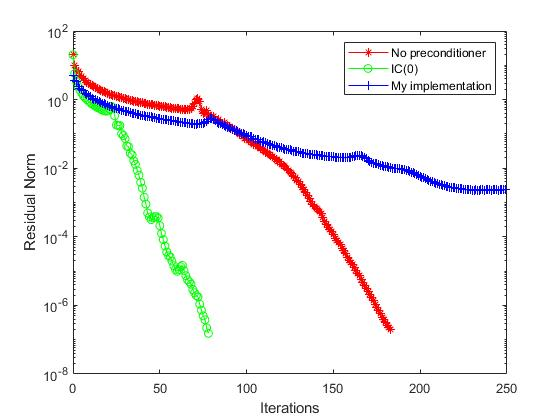
\includegraphics[width=.6\linewidth]{ex1_it250.jpg}
				\caption{Residual norm vs iteration number for PCG methods, $maxit=250$}
				\label{fig:ex1_it250}
			\end{figure}
		
			\begin{table}[H]
				\centering
				\begin{tabular}{c|c|c|c}
					\textbf{Method} 					&  \textbf{Iterations} 	& \textbf{Final Residual} 		& \textbf{Computational Time} 	\\ \hline
					Matlab PCG without preconditioning	& 			$183$ 		& $ 1.9591 \times 10^{-7} $ 	& $ 0.077 s $					\\ \hline
					Matlab PCG IC(0)					& 			$78$ 		& $ 1.5293 \times 10^{-7} $ 	& $ 0.068 s $					\\ \hline	
					My PCG implementation				& 			$250$		& $ 2.3 \times 10^{-3} $		& $	0.151 s $					\\
				\end{tabular}
				\caption{Results of PCG methods, $maxit=250$}
				\label{table:ex1_it250}
			\end{table}
		
			When $ maxit $ is large enough to guarantee convergence in all implementations we get the following results:
			\begin{figure}[H]
				\centering
				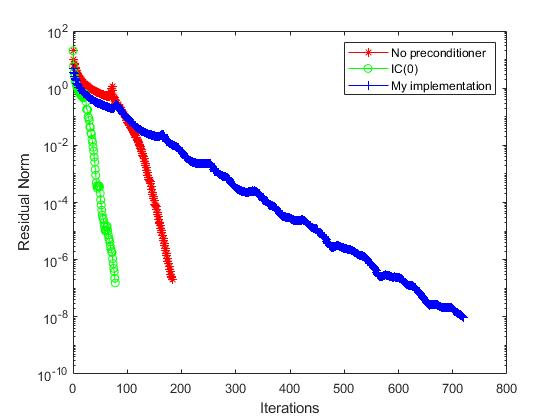
\includegraphics[width=.6\linewidth]{ex1_it750.jpg}
				\caption{Residual norm vs iteration number for PCG methods, $maxit=750$}
				\label{fig:ex1_it750}
			\end{figure}
		
			\begin{table}[H]
				\centering
				\begin{tabular}{c|c|c|c}
					\textbf{Method} 					&  \textbf{Iterations} 	& \textbf{Final Residual} 		& \textbf{Computational Time} 	\\ \hline
					Matlab PCG without preconditioning	& 			$183$ 		& $ 1.9591 \times 10^{-7} $ 	& $ 0.054 s $					\\ \hline
					Matlab PCG IC(0)					& 			$78$ 		& $ 1.5293 \times 10^{-7} $ 	& $ 0.063 s $					\\ \hline	
					My PCG implementation				& 			$720$		& $ 9.6833 \times 10^{-9} $		& $	0.351 s $					\\
				\end{tabular}
				\caption{Results of PCG methods, $maxit=750$}
				\label{table:ex1_it750}
			\end{table}
			
			My implementation is slower to converge but produces better final residual values.
			
			
		\section*{Question 2}
			The spectral condition number of A is 
			
			\begin{equation}
				\kappa(A) = \frac{\lambda_{max}(A)}{\lambda_{min}(A)}.
			\end{equation}
		
			In Matlab I used the \texttt{condest(A)} function to estimate the condition number of a sparse matrix A.
		
			\begin{table}[H]
				\centering
				\begin{tabular}{c|c|c|c|c|c|c|c}
					$n_x$   & $ h $						& $\kappa(A)$			 & $ \sqrt{\kappa(A)} $& $ CG $ & $ PCG(0) $& $PCG(10^{-2})$& $PCG(10^{-3})$ \\ \hline
					$ 102 $ & $ 1.0000 \times 10^{-4} $ & $ 6.0107 \times 10^3 $ & $ 77.5288 $ 		& $ 283 $ 	& $ 87 $ 	& $ 45 $ 		& $ 17 $ 		\\ \hline
					$ 202 $ & $ 2.5000 \times 10^{-5} $ & $ 2.3810 \times 10^4 $ & $ 154.3039 $ 	& $ 532 $ 	& $ 159 $ 	& $ 78 $ 		& $ 30 $ 		\\ \hline
					$ 402 $ & $ 6.2500 \times 10^{-6} $ & $ 9.4770 \times 10^4 $ & $ 307.8473 $ 	& $ 948 $ 	& $ 282 $ 	& $ 137 $ 		& $ 53 $		\\ \hline
					$ 802 $ & $ 1.5625 \times 10^{-6} $ & $ 3.7814 \times 10^5 $ & $ 614.9304 $ 	& $ 1792 $	& $ 533 $ 	& $ 258 $ 		& $ 97 $ 		\\ 
				\end{tabular}
				\caption{Iterations of PCG methods for each value of $n_x$ and respective values of $h$ and $\kappa(A)$}
				\label{table:ex2}
			\end{table}	
		
			One can note from the table the dependence of the number of iterations on $ h = \frac{1}{N} = \frac{1}{(nx-2)^2} $.
			The number of iterations is halved when $n_x$ approximately doubles.		
			
				
		\section*{Question 3}
			show theoretically ??
			
			When using the Choledsky precontionier with no fill in, I did'nt get the expected results.
			Both Matlab's and my implementation converged in only one iteration.
			
			\begin{figure}[H]
				\centering
				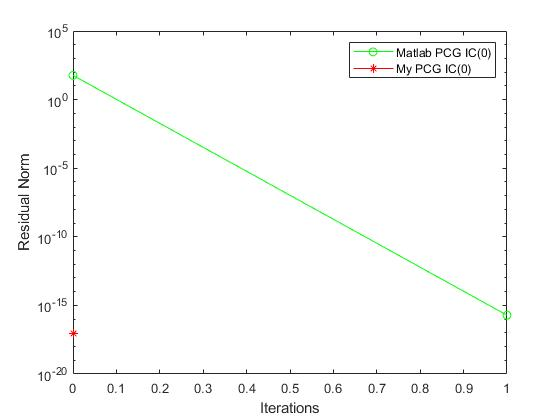
\includegraphics[width=.6\linewidth]{ex3.jpg}
				\caption{Residual norm vs iteration number for PCG methods with $IC(0)$ preconditioner}
				\label{fig:ex3}
			\end{figure}
		
			
			Due to the bad results, I tried to remove preconditioning form my implementation by setting $L$ as the identity matrix, \texttt{L = speye(size(L))}.
			\begin{figure}[H]
					\centering
					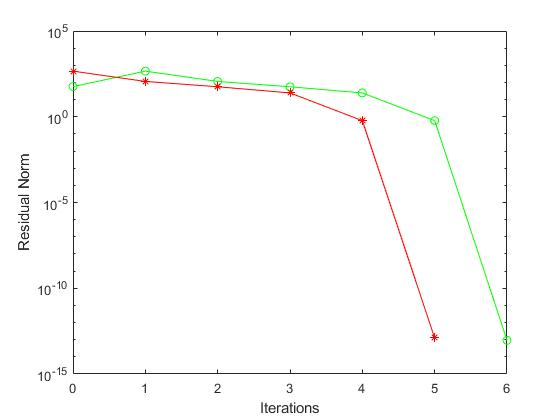
\includegraphics[width=.6\linewidth]{ex3_NoPrec.jpg}
					\caption{Residual norm vs iteration number for PCG methods without preconditioning}
					\label{fig:ex3_NoPrec}
			\end{figure}
		
			\begin{table}[H]
				\centering
				\begin{tabular}{c|c|c|c}
					\textbf{Method} &  \textbf{Iterations} 	& \textbf{Final Residual} 		& \textbf{Computational Time} 	\\ \hline
					Matlab PCG		& 			$6$ 		& $ 9.2128 \times 10^{-14} $ 	& $ 0.021 s $	\\ \hline	
					My PCG 			& 			$5$			& $ 1.2744 \times 10^{-13} $	& $	0.012 s $	\\ \hline
				\end{tabular}
				\caption{Results for each value of implementation, no preconditioning}
				\label{table:ex3_NoPrec}
			\end{table}
			These results show the theoretical calculations, my implementation is still better than expected.
			
		
		
		
		\section*{Question 4}		
			\begin{figure}[H]
				\centering
				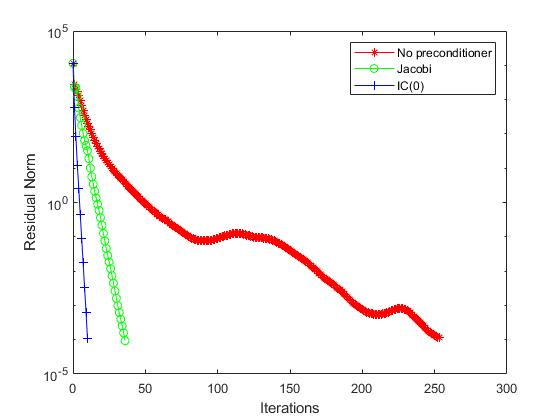
\includegraphics[width=.6\linewidth]{ex4.jpg}
				\caption{Residual norm vs iteration number for PCG methods without preconditioning}
				\label{fig:ex4}
			\end{figure}
		
			\begin{table}[H]
			\centering
			\begin{tabular}{c|c|c|c}
				\textbf{Preconditioner} &  \textbf{Iterations} 	& \textbf{Final Residual} 		& \textbf{Computational Time} 	\\ \hline
				None					& 			$253$ 		& $ 1.1367 \times 10^{-4} $ 	& $ 0.254 s $	\\ \hline
				Jacobi					& 			$36$ 		& $ 9.3198 \times 10^{-5} $ 	& $ 0.053 s $	\\ \hline		
				IC(0)					& 			$10$		& $ 1.1155 \times 10^{-4} $		& $	0.046 s $	\\
			\end{tabular}
			\caption{Results for each preconditioner}
			\label{table:ex4}
			\end{table}
		
		There is a very clear improvement when using preconditioning.
		It is also noticeable the superior characteristics of the incomplete Choledsky preconditioner relative to Jacobi.
		
		\section*{Question 5}
		
		
		\section*{Question 6}
		\begin{figure}[H]
			\centering
			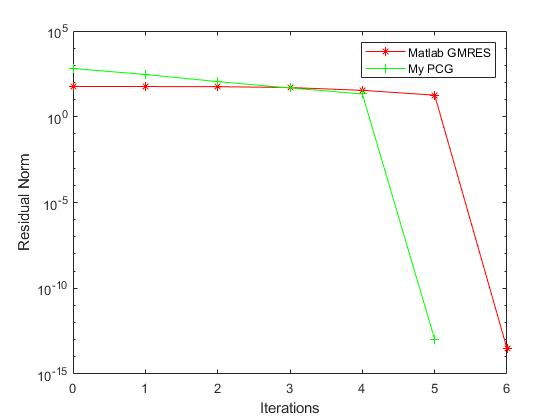
\includegraphics[width=.6\linewidth]{ex6.jpg}
			\caption{semilogy plot ex6}
			\label{fig:ex6}
		\end{figure}
		
		4.5350e-13
		
		7.1893e-14
		
			
		
		With L
		
		\begin{table}[H]
			\centering
			\begin{tabular}{c|c|c|c}
				\textbf{Method} &  \textbf{Iterations} 	& \textbf{Final Residual} 		& \textbf{Computational Time} 	\\ \hline
				GMRES 			& 			1 			& $ 3.8481 \times 10^{-16} $	& $ 0.027 s $	\\ \hline	
				My PCG 			& 			1			& $ 1.7554 \times 10^{-17} $	& $ 0.003 s $	\\ \hline
			\end{tabular}
			\caption{Iterations for each value of nx}
			\label{table:ex4_c_prec}
		\end{table}	
	
		GMRES without preconditioning, My PCG with L as identity matrix
			
		\begin{table}[H]
			\centering
			\begin{tabular}{c|c|c|c}
				\textbf{Method} &  \textbf{Iterations} 	& \textbf{Final Residual} 		& \textbf{Computational Time} 	\\ \hline
				GMRES			& 			$6$ 		& $ 3.0413 \times 10^{-14} $ 	& $ 0.102 s $	\\ \hline	
				My PCG 			& 			$5$			& $ 1.0468 \times 10^{-13} $	& $ 0.012 s $	\\ \hline
			\end{tabular}
			\caption{Iterations for each value of nx, no preconditioning}
			\label{table:ex4_c_NoPrec}
		\end{table}
	
		\begin{figure}[H]
			\centering
			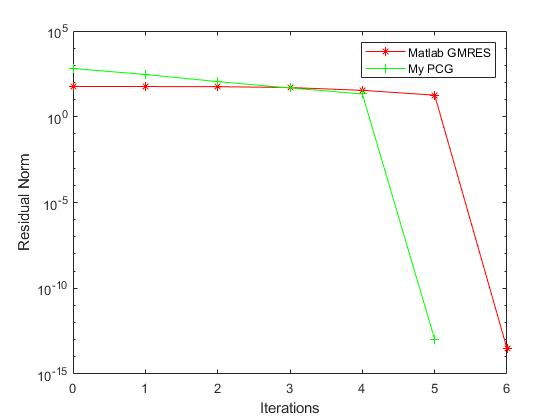
\includegraphics[width=.6\linewidth]{ex6b.jpg}
			\caption{semilogy plot ex6, GMRES without preconditioning, My PCG with L as identity matrix}
			\label{fig:ex6_c_NoPrec}
		\end{figure}
		
		
		
		\section*{Question 7}
		
		\begin{table}[H]
			\centering
			\begin{tabular}{c|c|c|c}
				\textbf{Restart} &  \textbf{Iterations} 	& \textbf{Final Residual} 		& \textbf{Computational Time} 	\\ \hline
				10			& 			$1149$ 		& $ 9.6915 \times 10^{-13} $ 	& $ 2.235 s $	\\ \hline	
				20			& 			$739$		& $ 9.6140 \times 10^{-13} $	& $ 1.443 s $	\\ \hline
				30			& 			$88$ 		& $ 6.7203 \times 10^{-13} $ 	& $ 0.242 s $	\\ \hline	
				50			& 			$41$		& $ 4.8414 \times 10^{-13} $	& $ 0.135 s $	\\ \hline
			\end{tabular}
			\caption{Iterations for each value of nx, no preconditioning}
			\label{table:ex7}
		\end{table}
		
		\begin{figure}[H]
			\centering
			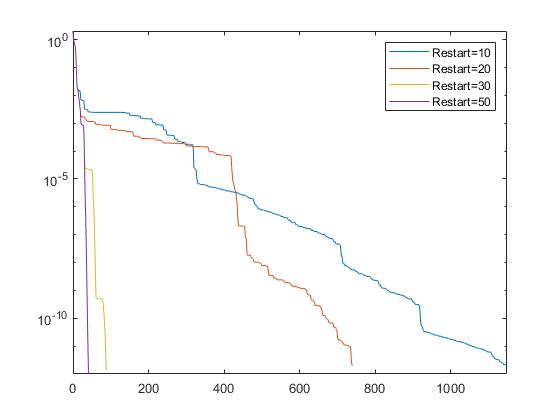
\includegraphics[width=.6\linewidth]{ex7.jpg}
			\caption{semilogy plot ex7}
			\label{fig:ex7}
		\end{figure}
	
		
		\section*{Question 8}
		
		\begin{table}[H]
			\centering
			\begin{tabular}{c|c|c|c|c|c|c}
				\textbf{Tolerance} & \textbf{Iterations} & \textbf{Tprec}  & \textbf{Tsol}  & \textbf{Ttotal} & \textbf{Final Residual} & \textbf{rho} \\ \hline
				$2 \times 10^{-2}$ & $1983$	& $ 39.59 s $ 	& $ 77.65 s $ & $ 117.24 s $ 	& $ 9.9053 \times 10^{-13} $ & $ 0.4537 $\\ \hline
				$1 \times 10^{-2}$ & $691$	& $ 36.46 s $ 	& $ 26.63 s $ & $ 63.09 s $ 	& $ 9.7254 \times 10^{-13} $ & $ 0.5807 $\\ \hline
				$3 \times 10^{-3}$ & $247$	& $ 40.67 s $ 	& $ 11.04 s $ & $ 51.71 s $ 	& $ 9.1709 \times 10^{-13} $ & $ 0.9401 $\\ \hline
				$1 \times 10^{-3}$ & $102$	& $ 37.61 s $ 	& $ 5.63 s $ & $ 43.24 s $ 		& $ 8.7501 \times 10^{-13} $ & $ 1.4544 $\\ \hline
				$1 \times 10^{-4}$ & $34$	& $ 42.44 s $ 	& $ 2.93 s $ & $ 45.37 s $ 		& $ 4.5169 \times 10^{-13} $ & $ 3.5140 $\\ \hline
				$1 \times 10^{-5}$ & $16$	& $ 76.50 s $ 	& $ 2.49 s $ & $ 78.99 s $ 		& $ 4.9947 \times 10^{-13} $ & $ 9.0720 $\\ \hline
			\end{tabular}
			\caption{Iterations for each value of nx, no preconditioning}
			\label{table:ex8}
		\end{table}
	
		
		
		\begin{figure}[H]
			\centering
			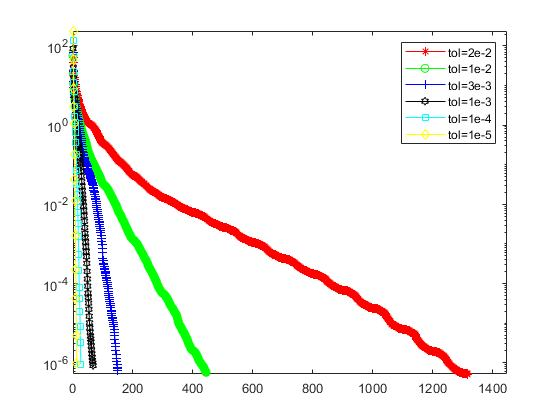
\includegraphics[width=.6\linewidth]{ex8.jpg}
			\caption{semilogy plot ex8}
			\label{fig:ex8}
		\end{figure}
	
	
	
\end{document}



